\documentclass[a4paper, justified,marginals=raggedright]{tufte-handout}


\usepackage[utf8]{inputenc}
\usepackage{graphicx} % allow embedded images
  \setkeys{Gin}{width=\linewidth,totalheight=\textheight,keepaspectratio}
  \graphicspath{{graphics/}} % set of paths to search for images
\usepackage{amsmath}  % extended mathematics
\usepackage{amssymb}  % more math symbols
\usepackage{booktabs} % book-quality tables
\usepackage{units}    % non-stacked fractions and better unit spacing
\usepackage{multicol} % multiple column layout facilities
\usepackage{fancyvrb} % extended verbatim environments
  \fvset{fontsize=\normalsize}% default font size for fancy-verbatim environments
\usepackage{pgfplots}

\usepackage{lipsum}

% to see the margins and page width
% \geometry{showframe}

% Write packages versions in the log
% \listfiles


% Commands use to make the title page and page headers
\title{Why and how to craft a trade-of in a plant functioning model}
\author{Clément Viguier}

% Commands use through the document


% Include documents for graphical aspects
% Color
%\input{../latex_settings/colors}
% Graph settings
\pgfplotsset{compat=newest}

\pgfplotsset{plot/.style={ 
width = \textwidth,
no markers,
color = black,
line width = 1pt,
minor x tick num = 0,
minor y tick num = 0,
        xtick pos=left,
        ytick pos=left,
        tick align=outside,
        try min ticks=2,
        max space between ticks=100pt,
  axis x line*=bottom,
  axis y line*=left,
        line join=round,
    axis line style={->}, 
        enlarge x limits=true,
        every x tick/.style={color=black, thin},
        every y tick/.style={color=black, thin},
}
}


\pgfplotsset{marginplot/.style={ 
plot,
width = \marginparwidth
}
}

\pgfplotsset{fullplot/.style={ 
plot,
width = \pagewidth
}
}

\begin{document}
\maketitle
\begin{fullwidth}
\begin{abstract}
\noindent
This document describes why and how a trade-of has be designed in the model MountGrass. This trade-of has the objective to allow for different strategy based on the level of resources. The same trade-of is used in shoot and roots. Parameters effects over the phenotype determination is explored for a balanced design where area cost is the same for both organs.
\end{abstract}
\end{fullwidth}

\section{Why a trade-of}
different conditions = different phenotypes\\
could be anything, needed one. Explain WUE, nitrogen and others. Try to keep independences between strategy axis to keep it simple.\\
Need for plastic driver. Explain the role of plasticity.

\section{How to craft a trade-of}

\indent The idea of trade-of suggest that you cannot invest in all strategies at the same time. To be relevant, it must be associated to a range conditions favouring different strategies along this trade-of. In other word, depending on a position on a gradient, the gradient should lead different niches. This can be visualizes as Gaussian's curves (see figure \ref{fig:niches}).

\begin{marginfigure}[-30mm]
\begin{tikzpicture}
\begin{axis}[marginplot,
legend style
={at={(1, 1.1)},
anchor=south east,
draw = none},
samples = 40]

\addplot[teal][domain = 0:1 ] {exp(-(x - 0.4)^2/0.02)};
\addplot[orange][domain = 0:1 ]{exp(-(x - 0.6)^2/0.02)};
\legend{Conditions 1, Conditions 2, Conditions 3}
\end{axis}
\end{tikzpicture}
\label{fig:niches}
\caption{Different niches corresponding to different environmental conditions.}
\end{marginfigure}

The challenge is to go beyond the Gaussian function, and craft these niches from the plant physiology and ecology. Taking as a basis the usual functions used in plant modelling and the theoretical background upon which MountGrass is built, we will try to model different niches.\\

\indent In MountGrass, the Leaf Economic spectrum (LES)\cite{Wright-2004} is explained by a differential investment between active and structural tissues (supported by analysis of Shipley\cite{Shipley}). This allocation constitutes a major strategic differentiation axis, along which plastic plants can move to optimize their fitness. To keep the approach simple, we hypothesize that such trade-off would also rule the allocation of organic matter in the below-ground compartment\cite{Reich-2014; Tjoelker-2005}. As explained above, plant can modify both the shot:root ratio, and the relative proportion of active tissues in shoot, and in roots. The first dimension is mainly driven by a balance between availability of above-ground versus below-ground resource.\footnote{This part does not belong to this section.}\\
\subsection{Crafting a trade-of for shoot}
\indent Let's consider only the shoot dimension for now, the demonstration that the same applies to root is done latter in the document.\\
\indent The fitness function of the shoot can be described as the sum of the gain function and the cost function as follow:
\begin{equation}\label{eq:gain}
Net~Gain = \frac{Exchange}{Area} . \frac{Area}{Biomass} - \frac{Resp}{Biomass}
\end{equation}
where $\frac{Exchange}{Area}$ is the resource mass exchanges per area (function of exchange rate and resource availability), $\frac{Area}{Biomass}$ is the SLA (or inverse of leaf construction cost) and $\frac{Resp}{Biomass}$ is the normalize biomass \footnote{The temporal dimension of the LES is ignored as the parameters are chosen for a fitness equivalence on the construction cost-lifespan trade-of.}. Let's analyse how these variables vary for a constant level of resources with the relative proportion of active tissue. For convenience the exchange rate is assumed to be constant for the following calculations.
The SLA is the inverse function of the leaf density. If we consider that active and structural tissue pools are two distinct constant densities respectively noted $\rho_{act}$ and $\rho_{str}$ with $\rho_{act} < \rho_{str}$, the leaf area per carbon unit can be written:
\begin{equation} \label{eq:SLA}
SLA = \frac{1}{th. vol_prop} \left(\frac{1}{\rho_{str}}+\left(\frac{1}{\rho_{act}}-\frac{1}{\rho_{str}}\right)p_{act}\right)
\end{equation}
where $th$ is the thickness of the leaf, $vol_prop$ is the proportion of leaf volume occupied by tissue and $p_{act}$ is the fraction of active tissue. This shows a linear relationship between the gain function ($SLA . exchange_rate$) and the proportion of active tissue ($p_{act}$).


\begin{marginfigure}[-30mm]
\begin{tikzpicture}
\begin{axis}[marginplot,
legend style
={at={(1, 1.1)},
anchor=south east,
draw = none},
samples = 40,
restrict y to domain=-2000:2000,
xlabel = $p_{act}$]

\addplot[teal][domain = 0:1 ] {(1/(0.022 * 1)) * (1/1 + (1/0.05 - 1)*x)};
\addplot[orange][domain = 0:1 ] {exp(7*x) + 0.03*x};
\legend{$\frac{Exchange}{Area}\frac{Area}{Biomass}= f(p_{act})$, $e^{kx} + r_{1}p_{act}$}
\end{axis}
\end{tikzpicture}
\label{fig:gain_cost}
\caption{Comparison of "gain" function and "cost" function. Parameter values: $\rho_{act} = 0.05$, $\rho_{str} = 1$,  $k = 7$ and  $vol_prop = 1$. The area between the two curves is the total gain by the plant.}
\end{marginfigure}



On figure \ref{fig:gain_cost} we see that the difference between the gain and cost functions leads to a bumpy curve with a maximum. This difference is the net gain and it admits a maximum corresponding to optimum value for $p_{act}$. The gain function (equation \ref{eq:gain}) can be rewritten with equations use to trace figure \ref{fig:gain_cost}. Plus, in the context of the model, the exchange rate is function of the resource availability, maximum exchange rate and the day length. This can be stored in one variable that will define the external conditions note $R$. From this the new gain function look like that.
\begin{align}\label{eq:net_gain}
Net~Gain & = R\frac{1}{th . vol_prop} \left(\frac{1}{\rho_{str}}+\left(\frac{1}{\rho_{act}}-\frac{1}{\rho_{str}}\right)p_{act}\right) - (exp^{k.p_{act}} + r_{1}p_{act})\\
& =R (g_{1} + g_{2}p_{act}) - (e^{k.p_{act}} + r_{1}p_{act}) \\
\end{align}

From this, it is possible to compute $p_{act}$ to have the maximum net gain. The first derivatives of this function are easy to calculate and come as follow:

\begin{equation}\label{eq:net_gain_der}
f'(p_{act}) = R.g_{2}p_{act} - (k.e^{k.p_{act}} + r_{1})
\end{equation}
but the equation $f'(p_{act}) = 0$ is not numerically solvable, but we can visualize that the net gain function have different maximum for $p_{act}$ in the interval $[0:1]$.


\begin{figure}
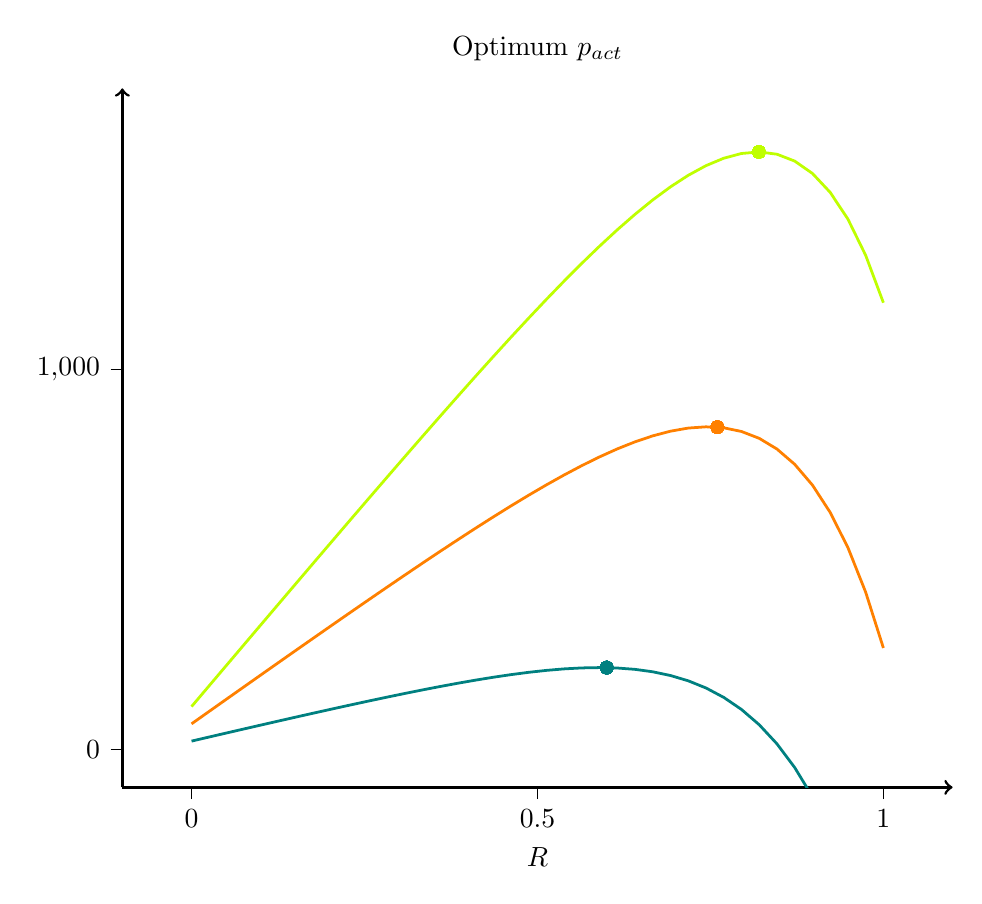
\begin{tikzpicture}
\begin{axis}[plot,
legend style
={at={(1, 0.1)},
anchor=south east,
draw = none},
samples = 40,
restrict y to domain=-2000:2000,
title = Optimum $p_{act}$,
xlabel = $R$,
ymin = -100]

% R*( g1 + g2 p_act ) − ( e(k.p_act)+ r1 .p_act )
% g1 = 1:(th*vt_s) * (1/tho_ss) = 1/0.022
% g2 = 1:(th*vt_s) * (1/rho_as - 1/tho_ss) = 1/0.022 * (1/0.05 - 1)
\addplot[teal][domain = 0:1 ] {0.5 * 1/0.022 * (1+(1/0.05 - 1)*x) - (exp(7*x) + 0.03*x)};
\addplot[orange][domain = 0:1 ] {1.5 * 1/0.022 * (1+(1/0.05 - 1)*x) - (exp(7*x) + 0.03*x)};
\addplot[lime][domain = 0:1 ] {2.5 * 1/0.022 * (1+(1/0.05 - 1)*x) - (exp(7*x) + 0.03*x)};
\addplot[teal][domain =  0.6:0.6001, only marks]{0.5 * 1/0.022 * (1+(1/0.05 - 1)*x) - (exp(7*x) + 0.03*x)};
\addplot[orange][domain =  0.76:0.76001 , only marks]{1.5 * 1/0.022 * (1+(1/0.05 - 1)*x) - (exp(7*x) + 0.03*x)};
\addplot[lime][domain =  0.82:0.82001, only marks]{2.5 * 1/0.022 * (1+(1/0.05 - 1)*x) - (exp(7*x) + 0.03*x)};
\end{axis}
\end{tikzpicture}
\label{fig:optimum}
\caption{$\blacktriangleleft$ Comparison of "gain" function and "cost" function. Parameter values: $g_{2} = $, $g_{2} = $,  $k = 7$}
\end{figure}


\begin{marginfigure}[-63mm]
\begin{tikzpicture}
\begin{axis}[marginplot,
legend style
={at={(1, 1.1)},
anchor=south east,
draw = none},
samples = 40,
restrict y to domain=-300:700,
xlabel = $p_{act}$,
extra x ticks={0.618},
extra x tick style={grid=major}]

\addplot[darkgray][domain = 0:1 ] {(1/(0.022 * 1)) * (1 + (1/0.05 - 1)*x) - (exp(7*x) + 0.03*x)};
\addplot[gray][domain = 0:1 ] {(1/(0.022 * 1)) * ((1/0.05 - 1)*x) - (7*exp(7*x) + 0.03)};
\legend{$Net~gain$, $f'$}
\end{axis}
\end{tikzpicture}
\label{fig:derivaives}
\caption{Net gain function and its first derivative.} Looks like there is some kind of mismatch here.
\end{marginfigure}

\subsection{How about root}

\subsection{How do the two trade-of merge ?}


\end{document}